\part*{Lecture 7: Volatility Skew and the SABR Model}
\addcontentsline{toc}{part}{Lecture 7: Volatility Skew and the SABR Model}
\beginlecture{07}

The lecturer opened Lecture~7 with a long, deliberate recap of caps,
floors, and swaptions --- the entire first hour of the session was spent
not on new material but on re-anchoring why caps, floors, and swaptions
exist as products, what their implied vols are quoting, and how those
vols connect back to bond-pricing intuitions from Week~1. Only after a
short break did he pivot to today's actual headline topic: the
\emph{volatility skew}, the empirical fact that Black's implied vol is
not constant across strikes, and the \textbf{SABR model} that fixed-income
desks use to fit and extrapolate that skew.

The structural picture the lecturer wanted in our heads by the end of
the lecture is this. Caps, floors, swaptions, and STIR-future options
are quoted in implied vol because vol is the apples-to-apples language
across products, exactly the way YTM is for bonds. But just as YTM is
not a deep object --- the spot curve underneath is --- implied vol is
not a deep object: an entire surface of forward vols underneath it is.
Lecture~6 built the bootstrap from flat caplet vols to forward vols
along the \emph{tenor} axis. Lecture~7 turns to the \emph{strike} axis:
at any one tenor, the cross-section of implied vols against strike is
the \emph{skew}, and SABR is the workhorse model that gives a stochastic-vol
explanation for the skew, an arbitrage-free closed-form approximation
for it, and --- the part that matters most for hedging --- a
\emph{prediction of how the skew shifts when the underlying moves}.
That last piece is what the lecturer kept calling the
\textbf{Vega channel}, and it is the reason a market-maker on a large
fixed-income book cannot simply rely on Black's $\Delta$.

\section{Why caps, floors, and swaptions matter (recap)}\label{L7-sec:recap}

The first half-hour of the lecture had the lecturer asking the class
to remind him, in their own words, why caps, floors, and swaptions
exist as standalone products. The structure of the recap was the same
``call/put toolkit'' lens introduced in Lecture~6, but the lecturer
sharpened a few framings that are worth keeping.

\subsection{Swaps as a duration-transformation primitive}\label{L7-sec:swaps-recap}

\begin{keyblock}
\textbf{Cells (Page \emph{Vol Skew} setup recap).}
\emph{(Why swaps are a foundational fixed-income product.)}\\
A swap decomposes as
\[
  \text{receive-fixed swap}
     \;=\; (\text{long fixed coupon bond}) \;-\; (\text{short floating-rate bond}),
\]
and the fixed leg of a 10-year swap inherits the duration of a 10-year
coupon bond ($\sim 7$--$8$~years), while the floating leg has near-zero
duration (it resets to par every period). \textbf{Receiving fixed adds
duration; paying fixed subtracts.} Swaps are therefore the
``magical duration transformation'' a portfolio overlay desk uses to
move duration without trading the underlying bonds.
\end{keyblock}

The lecturer pushed against the most common student framing of swaps
--- ``a coincidence of wants where two parties want each other's coupon
type.'' That framing is real but not the punchline:
``what you said is that the swaps were managing duration. Why is that?
Because the swap could be decomposed into\ldots\ a fixed and floating
rate bond.'' The lesson he wanted recorded is that swaps are not in the
top-three OTC products because of issuer-investor preference matching;
they are there because they let any large book reshape duration
cheaply.

\subsection{Forward swaps and swaptions as the next layer}\label{L7-sec:swaptions-recap}

\begin{keyblock}
\textbf{Cells (recap of \emph{Swaptions} from Lecture~6).}
\emph{(Two layers of optionality on top of the spot swap.)}
\begin{itemize}
  \item A \textbf{forward swap} locks in today the swap rate at which
        the parties will enter a swap at some future date $T_o$. Its
        contract value at inception is zero when struck at the
        \emph{forward swap rate} $f_n(0,T_o,T)$.
  \item A \textbf{payer swaption} is a \emph{call} on the forward swap
        rate; a \textbf{receiver swaption} is a \emph{put}.
        Put--call parity:
        \[
          p_{\text{payer}}(K) \;-\; p_{\text{receiver}}(K)
            \;=\; (\text{forward swap struck at } K),
        \]
        so at $K = f_n(0,T_o,T)$ the swaption pair has zero value
        difference and the swaption itself is at-the-money in the
        Black-formula sense.
\end{itemize}
\end{keyblock}

The lecturer's framing here was equity-options-by-analogy. ``The
swaption is just going to be just like in equities. You could buy
Tesla.\ You could buy Tesla forward.\ We don't talk about that a lot
in equities.\ That's more important here in fixed income, the forward
pricing.'' Just as equity options on Tesla are the call/put toolkit on
the underlying Tesla share, swaptions are the call/put toolkit on
forward swaps. And just as caps and floors are the call/put toolkit on
spot swaps, swaptions extend it onto the \emph{forward}-swap layer
that sits above.

The four-by-four grid that the lecturer kept returning to:

\begin{keyblock}
\textbf{The structural grid.}
\begin{center}
\begin{tabular}{l|l}
\textbf{Spot world (caps/floors)} & \textbf{Forward world (swaptions)} \\
\hline
single-period option = caplet/floorlet & single option = swaption \\
strip of period options = cap/floor & one option on the bundle = swaption \\
long cap $-$ short floor $=$ \emph{spot} swap & long payer $-$ short receiver $=$ \emph{forward} swap \\
ATM $\Leftrightarrow$ $K = $ spot swap rate & ATM $\Leftrightarrow$ $K = $ forward swap rate \\
\end{tabular}
\end{center}
\end{keyblock}

The lecturer also re-stated the option-on-portfolio-vs-portfolio-of-options
distinction. A cap is a portfolio of caplets: the holder picks and
chooses which caplets to exercise period-by-period. A swaption is one
option on a portfolio: the holder commits to the entire underlying
swap with one exercise decision at $T_o$. With matching strikes and
notionals, the cap or floor is therefore worth weakly more than the
swaption. Different products for different uses: caps and floors when
you want optionality on each individual cash flow, swaptions when the
question is whether to enter a forward swap at all.

\begin{checkpoint}
\textbf{My note.} The lecturer wanted us to internalize the lens that
\emph{every fixed-income optional product is the call/put toolkit on
some underlying rate or rate-bundle}. That is why these products dwarf
their equity counterparts: the underlyings (spot swaps, forward swaps)
are themselves enormous markets whose participants demand asymmetric,
non-linear exposures. ``We have the puts and the calls, in this case,
being payer swaptions and receiver swaptions, are going to build out
those forward swap rates.'' Once the lens is in place, the formulas
are rote: Black's call on the right forward, scaled by the right
discount factor (single $Z(0,T_o)$ for caplets, swap discount factor
$\sum_i Z(0,T_i)$ for swaptions).
\end{checkpoint}

\subsection{Flat vol and forward vol as YTM and spot rate}\label{L7-sec:flatvfwd-recap}

\begin{keyblock}
\textbf{The two implied-vol layers (recap).}
\begin{center}
\begin{tabular}{l|l}
\textbf{Bond pricing} & \textbf{Cap pricing} \\
\hline
YTM (one number per bond) & flat vol (one number per cap) \\
prices the bundle, not each cash flow & prices the cap, not each caplet \\
spot rates (one per maturity, consistent) & forward vols (one per tenor, consistent) \\
extracted by bootstrap from YTMs & extracted by bootstrap from flat vols \\
\end{tabular}
\end{center}
\end{keyblock}

The lecturer used this slide to surface two practical points.
First, that the cap-bootstrap is a much cleaner story than the
Treasury-bootstrap: ``when I go to those main market makers [of caps],
they are ready and available to quote me at any of these maturities.''
Treasuries are an irregularly-issued grid; caps and floors are an OTC
grid the dealer fills on demand, so the bootstrap is exactly identified
maturity-by-maturity and recovers a sensible forward-vol curve without
any Nelson--Siegel-style smoothing.

Second, that the convexity-of-flat-vol diagnostic carries straight
over from spot/YTM. When the flat vol is rising in $T$, the new caplet
must have a forward vol \emph{higher} than the running flat vol to pull
the average up; when the flat vol is falling in $T$, the new caplet's
forward vol must be \emph{lower}. ``As I see these flat vols going up
and up and up, what do I know must be true of these caplet vols, of the
forward vols? They have to be even higher.''

\begin{tipblock}
\textbf{Filling the gap.} The lecturer flagged but did not labor the
naming-confusion the class always trips on: the cap analog of the
\emph{spot rate} (the consistent maturity-by-maturity object) is called
the \emph{forward vol}, not the spot vol. The reason is that the
caplet writes an option on a \emph{forward} rate (the forward rate
locked at $T - 1/n$ and paid at $T$), so the implied vol on it is the
implied vol of a forward. The naming is technically correct and
emotionally awkward.
\end{tipblock}

\subsection{The swaption Black formula and what to plug in}\label{L7-sec:swaption-blackrecap}

\begin{keyblock}
\textbf{Cells (recap of \emph{Black's formula for swaptions}).}
\emph{(One Black call on the forward swap rate, scaled by the swap
annuity.)}\\
For a payer swaption with expiration $T_o$ on an $n$-frequency swap of
tenor $T$ struck at rate $K$:
\[
  p_{\text{payer}}
     \;=\; \frac{100}{n}\,Z^{\text{swap}}(0, T_o, T)\,
        \Bigl[\, f_n\,\cN(d_1) \;-\; K\,\cN(d_2)\,\Bigr],
\]
\[
  Z^{\text{swap}}(0, T_o, T) \;\equiv\; \sum_{i = 1}^{m} Z(0, T_i),
  \qquad
  d_{1,2} \;=\;
       \frac{\ln(f_n / K) \pm \tfrac{1}{2}\,\sigma^2\,T_o}
            {\sigma\,\sqrt{T_o}}.
\]
\textbf{Two things to plug in carefully:} the underlying is the
\emph{forward swap rate} $f_n(0, T_o, T)$, not today's spot swap rate;
and the discount factor is the \emph{swap annuity}
$\sum_i Z(0, T_i)$, not the single discount factor at swaption
expiration.
\end{keyblock}

The lecturer made a point of how strange the swap-annuity discounting
should feel. ``Did you ever do an option that if you exercise it, it
pays a stream of cash flows? I don't recall you ever doing that.\ \ldots\
The fact that this still works so seamlessly should strike you as\ldots\
interesting.'' The honest justification --- a change of numeraire to
the annuity / swap measure under which the forward swap rate is a
martingale --- belongs to FINMAT~330 and a hypothetical
``FINM~37500 at 100~units'' that would cover Heath--Jarrow--Morton and
the Libor Market Model. In our setting the recipe is asserted: trust
that the swap annuity is a valid numeraire, plug the forward swap
rate into Black, scale by the annuity, and the Bloomberg quote
translates to a dollar price.

\begin{keyblock}
\textbf{The forward swap rate (recap).}
\[
  f_n(0, T_o, T) \;=\; n\,
        \frac{Z(0, T_o) \;-\; Z(0, T)}{\sum_{i = 1}^{m} Z(0, T_i)}.
\]
A ``$1Y \to 4Y$'' swaption needs the \textbf{1-year forward 4-year
swap rate}, not today's 4-year swap rate. The forward swap rate is
just a function of the discount curve --- no vol input is needed to
compute it.
\end{keyblock}

A worked numerical example the lecturer ran by hand: with a
$1Y \to 4Y$ swaption, the forward swap rate came out to about $3.27\%$;
a $-200$~bps strike (i.e., $K = 1.27\%$) priced to about \$7 of premium
per \$100 notional. ``If I can lock it in at 1.27, currently, that
would stack up to like I'm getting 2 percentage points better a year
for four years.\ I'm getting, in a sense, 8\% better than what the
market currently prices.'' Time value plus a small amount of optionality
on whether the option stays deeply in the money rationalizes the
\$7 premium against the roughly 8-percentage-point intrinsic edge.

\subsection{Black vs Bachelier: the normal-vol toggle}\label{L7-sec:normal-toggle}

\begin{keyblock}
\textbf{Cell (recap).} \emph{(Bloomberg's normal-vol convention.)}\\
Bloomberg quotes vols by default in the \emph{normal} (Bachelier) form,
with a toggle for \emph{lognormal} (Black). At-the-money:
\[
  \sigma_B \;\approx\; \sigma_N \,/\, f,
\]
where $f$ is the relevant forward rate. For OTM strikes the conversion
gets a SABR-style correction. For the homework, all data has been
pre-converted to Black quotes, so the conversion is one to internalize
but not to re-derive each time.
\end{keyblock}

The lecturer's pragmatic line on the modeling choice: ``whether
log-normal or normal is not totally obvious, which would be a better
model.'' At rates close to zero, lognormal piles probability mass at
low rates and forbids negatives; normal lets rates go negative (a
small price after the 2014--2021 negative-rate episode in EUR / JPY).
Internal pricing groups will use a more sophisticated model than
either; the choice of quoting language is just convention. ``You're
speaking the language of Black, turning it into dollars.''

\subsection{The collared and leveraged floater case studies}\label{L7-sec:collared}

Before the break the lecturer worked one more case to keep the
caps-and-floors machinery practical: a \emph{collared floater}, a
floating-rate corporate note whose coupon is bounded inside an
interval $[K_{\text{floor}}, K_{\text{cap}}]$.

\begin{keyblock}
\textbf{Cells (case study, \emph{Collared floater}).}
\emph{(Decomposition into floating + cap + floor positions.)}\\
A collared floater that pays the floating rate inside the collar can
be replicated as
\[
  \text{collared floater}
     \;=\; \text{long floater} \;+\; \text{long floor at } K_{\text{floor}}
        \;-\; \text{short cap at } K_{\text{cap}}.
\]
The \textbf{long floor} kicks in when the floating rate falls below
$K_{\text{floor}}$ (the issuer is forced to pay the floor level); the
\textbf{short cap} kicks in when the floating rate rises above
$K_{\text{cap}}$ (the issuer caps the coupon for the bondholder). With
the cap and floor priced via Black's formula, the entire structure is
priced.
\end{keyblock}

\begin{checkpoint}
\textbf{My note.} The lecturer plotted (sketch only) the collared
floater's price-vs-rate curve. Unlike the strict convex/negative-convex
shape of a vanilla bond or an option, the collared floater shows
\emph{both}:
\begin{center}
\begin{tikzpicture}[scale=0.95]
  \draw[->] (0,0) -- (8,0) node[right] {rate $r$};
  \draw[->] (0,0) -- (0,4.5) node[above] {price};
  \draw[thick,blue,smooth,domain=0.4:7.6,samples=80,variable=\x]
    plot ({\x},{
      2.6
      + 0.45 * exp(-((\x-2.0)*(\x-2.0))/0.6)
      - 0.55 * exp(-((\x-5.5)*(\x-5.5))/0.5)
      - 0.04*\x
    });
  \draw[dashed,gray] (2.5,0) -- (2.5,3.4) node[above,black,scale=0.85] {$K_{\text{floor}}$};
  \draw[dashed,gray] (5.0,0) -- (5.0,2.55) node[above,black,scale=0.85] {$K_{\text{cap}}$};
  \node[scale=0.8] at (1.2,3.5) {floor kicks in};
  \node[scale=0.8] at (6.6,1.85) {cap kicks in};
\end{tikzpicture}
\end{center}
Inside the collar the floater behaves like a pure floater (near-zero
sensitivity to rates). Below the floor strike the bond gains value
because the issuer is paying above-market coupons (positive convexity
on the bondholder side). Above the cap strike the bondholder loses
because the coupon is bounded above (negative convexity on the
bondholder side). Rates spiking 200--300~bps suddenly --- as in 2022 ---
moves the bond out of the collar's flat region and the implied
sensitivity to rates returns.
\end{checkpoint}

The lecturer connected the collared floater to a related, more
dangerous product: the \emph{leveraged inverse floater}, whose coupon
moves the wrong way relative to rates with leverage. Built from
``go long a fixed bond, short the cap, long the floor'' (or its sign-
flipped version), this product was at the heart of the 1994
\emph{Orange County bankruptcy}. The lecturer's framing: ``somebody
kind of got hooked on thinking they were getting free money by taking
a very speculative options bet,'' and a desk armed with the
caps-and-floors decomposition could have stress-tested the position
against a sudden rate spike and seen the catastrophe coming. The
homework will not assign the leveraged inverse floater; the collared
floater is the assigned case.

After this segment the lecturer paused for a 7-minute break and
pivoted into the new material.

\section{The volatility skew, in pictures}\label{L7-sec:skewpictures}

\begin{keyblock}
\textbf{Cell (Page \emph{Examples of Vol Skew}).}
\emph{(What an implied-vol-vs-strike chart shows.)}\\
For a fixed underlying contract and a fixed expiration, plot Black's
implied vol $\sigma$ on the $y$-axis against strike $K$ on the $x$-axis,
with separate series for puts and calls. A point on the chart is the
$\sigma$ that, plugged into Black's formula, recovers the market price
at that strike. \textbf{No model has been built yet} --- this is just
inverting Black's formula, the same way a YTM is just inverting the
bond pricing formula. The chart is a translation of market prices into
$\sigma$-units.
\end{keyblock}

\begin{keyblock}
\textbf{Cell~7 (Page \emph{Examples of Vol Skew}).} \emph{(Implied-vol
curves across futures markets and expirations.)}

\begin{center}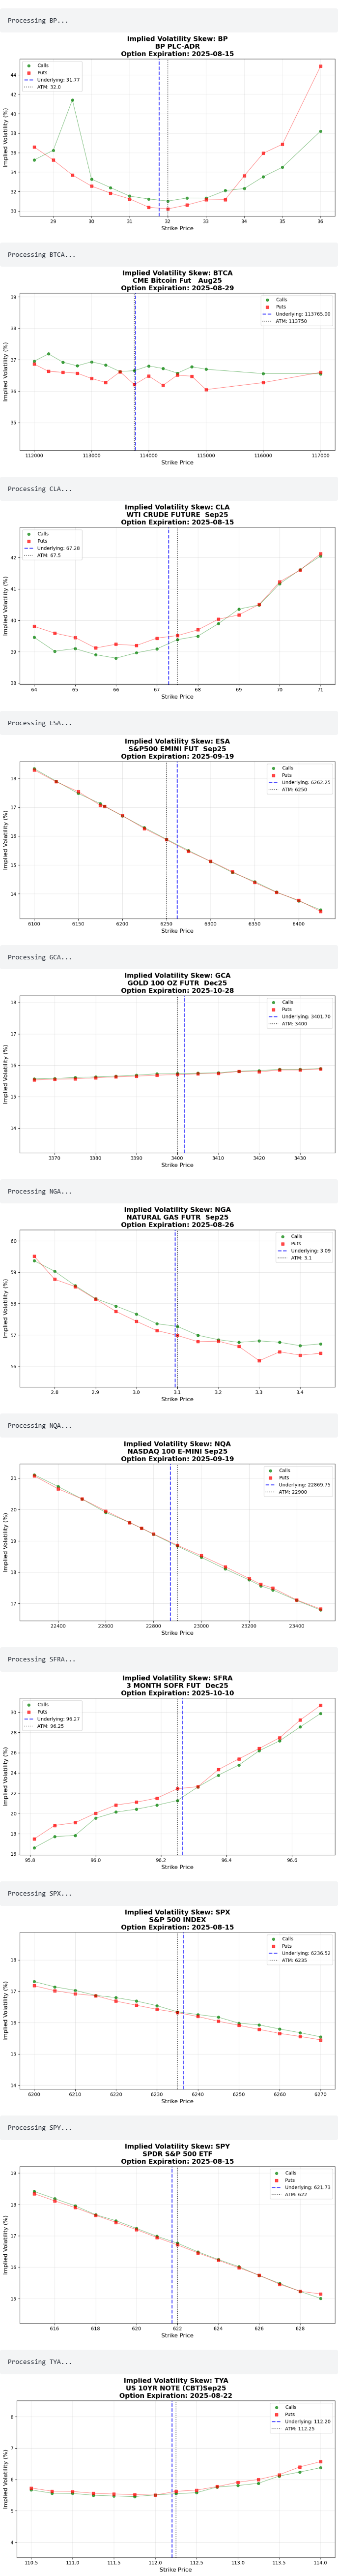
\includegraphics[width=0.8\linewidth,height=0.85\textheight,keepaspectratio]{figures/L7_1_c07_skew_examples.png}\end{center}

The notebook walks through implied-vol skews for several futures
contracts at various 2025 dates: WTI crude (CL), e-mini S\&P 500 (ES),
gold (GC), natural gas (NG), 3-month SOFR (SR3), 10-year Treasury
note futures (TY), and SPX index options. Each panel plots
\emph{calls} (one color) and \emph{puts} (another color) as separate
series of dots; both should lie on top of each other under Black, but
do not exactly. Some panels are smiles, some are smirks, some are
roughly flat.
\end{keyblock}

The lecturer used this slide to make the class state the obvious
facts and the not-so-obvious facts. Two students took the obvious
ones in turn:

\begin{quote}
\emph{Student:} ``It's basically mapping what the implied vol is for
different strike prices, different options. So for this one with
crude oil, the bigger shocks are kind of towards the upwards.''

\emph{Student:} ``It's basically you invert the Black formula to get
the implied vol for each point by looking at the market price.''
\end{quote}

The point the lecturer wanted on the table next was diagnostic:

\begin{keyblock}
\textbf{Two predictions if Black were exactly right.}
\begin{itemize}
  \item The dots would lie on a single \emph{flat horizontal line} ---
        the constant-volatility process Black assumes implies one
        $\sigma$ across all strikes.
  \item Calls and puts at the same strike would have \emph{identical}
        implied vols --- this is just put-call parity in
        $\sigma$-space.
\end{itemize}
We see neither. The flat-line failure is uncomfortable but tolerable:
``Black's formula is a translation, not a description of the world.''
The put-vs-call gap at a single strike is much harder to digest:
that one is internal inconsistency \emph{at the same strike}, which
ought to be tradable.
\end{keyblock}

\begin{tipblock}
\textbf{Filling the gap.} Why does put-call parity, in implied-vol
form, force the put and call IVs to coincide at a single strike? In
Black's world for futures with strike $K$, expiration $T$, discount
factor $Z(0,T)$, and forward $F = F(0,T)$, parity reads
\[
  C(K) \;-\; P(K) \;=\; Z(0,T)\,(F - K).
\]
The right-hand side is model-free and has no $\sigma$ in it. Plug
each side of the parity through Black's formula at separate $\sigma_C$
and $\sigma_P$:
\[
  Z(0,T)\bigl[F\,\cN(d_1^{(C)}) - K\,\cN(d_2^{(C)})\bigr]
  - Z(0,T)\bigl[K\,\cN(-d_2^{(P)}) - F\,\cN(-d_1^{(P)})\bigr]
  \;=\; Z(0,T)(F-K).
\]
Using $\cN(-x) = 1 - \cN(x)$, the equation simplifies and is consistent
\emph{iff} $\sigma_C = \sigma_P$. Any non-trivial gap is therefore a
parity violation in dollar terms, $C - P \ne Z(F - K)$.
\end{tipblock}

The lecturer made the class talk through why a parity violation is
not, in practice, a free lunch. Two answers came back: liquidity and
illiquidity-driven bid--ask. ``If you tried to build the put-call
parity arbitrage here, you'd have to worry that your own buying and
selling action are going to push through the bid-ask spread, and
you're going to actually not make anything.'' Black's formula
doesn't understand liquidity, so when the market needs to charge an
illiquidity premium it shows up as an implied-vol distortion. ``All
these vols are actually absorbing everything that Black's model fails
at. If it fails to understand liquidity, that's partly what this
picture is about.''

\subsection{Patterns across the example markets}\label{L7-sec:pattern-tour}

The lecturer walked the class through the panels in order. The
specific shapes are not laws of nature --- they shift day to day and
expiration to expiration --- but the snapshots illustrate the variety:

\begin{itemize}
  \item \emph{Crude oil (WTI), September~2025 contract, 2-months out.}
        Smirk skewed up at the high-strike side --- ``the bigger
        shocks are kind of towards the upwards.'' The lecturer noted
        this is opposite of the equity vol smirk most students will
        have seen in autumn.
  \item \emph{S\&P~500 e-mini, September contract, July pull date.}
        ``You may think this shape is surprising for the S\&P~500,
        but you should also recall that's going to differ based on the
        instrument and the expiration.'' The skew is mild for this
        short-dated future-on-future option; index-option skews for
        SPX options on cash settle differently.
  \item \emph{Gold and natural gas.} Gold near-flat. NG with high
        absolute IV levels (56--60\%) compared to e-mini's 18--30\%
        --- a useful reminder that ``vol'' is per-asset; you cannot
        compare cross-market levels naively.
  \item \emph{3-month SOFR future, options on the September contract.}
        Higher implied vol at high strikes, but the lecturer paused
        to remind the class of the strike convention: a STIR-future
        index level $96.5$ corresponds to a locked rate of
        $100 - 96.5 = 3.5\%$, so high strikes in index space are
        \emph{low} strikes in rate space. ``You'll see the same chart
        for STIR futures, where people will translate that strike into
        $100 - K$, well, then obviously the picture's going to flip.''
  \item \emph{10-year Treasury (TY) futures.} Notably flat across
        strikes. The implied vol level was around 6\% --- the small
        absolute number reflects that bond \emph{prices} have small
        vol (the tenor on the cheapest-to-deliver is only $\sim 8$
        years left) even when their underlying \emph{rates} have
        meaningful vol. The duration-rescaling between rate-vol and
        price-vol from Lecture~5 is the explanation.
\end{itemize}

\begin{checkpoint}
\textbf{My note.} The fact that the TY skew is so flat is interesting.
The lecturer kept it on screen for a beat: ``but I think anyone would
say the vol is pretty flat. What kind of vol are you getting on
treasuries? Very small numbers, right?\ Six percent annualized.''
Two-month-to-expiration option on a futures-contract that delivers a
cheapest-to-deliver Treasury whose remaining maturity is then
$\sim 8$ years --- the option's volatility absorbs all of those layers
and still comes out clean. This is one reason fixed-income desks
think the TY future is a much better signal for hedging than the
embedded-call apparatus on illiquid agency callables (Lecture~6).
\end{checkpoint}

\section{Why fit a model to the skew at all?}\label{L7-sec:whymodel}

After the picture-tour the lecturer asked the central pedagogical
question of the lecture: why bother fitting a model to that curve?
``You see there's a skew. You immediately start trying to model it
and you skip, well, why did we care?'' He pulled three reasons out
of the class, in increasing order of importance.

\subsection{Pricing the wings, as a market-maker}\label{L7-sec:wings}

\begin{keyblock}
\textbf{Reason 1: market-makers must quote where there is no recent data.}
At any moment, almost all option-market activity is at-the-money. If a
counterparty asks for a quote at $K$ that is $200$~bps OTM, the
market-maker has no recent trade and no recent quote at that strike.
She still has to quote.\\
The model is the device that says: \emph{given} the at-the-money quote
and the news (Fed governor speech, inflation print, oil shock), how far
should the OTM strike's vol be from the ATM vol \emph{today}?
\end{keyblock}

The lecturer's framing was concrete: ``There's been some news since
yesterday and no one's traded that strike in six hours. What are you
going to quote me?'' Without a model, the market-maker would simply
re-quote yesterday's far-OTM number, but yesterday's number does not
reflect today's news. With a model, the at-the-money information
propagates out to the wings via the model's structural assumptions.

\subsection{Inventory risk: my old positions drift OTM}\label{L7-sec:inventory}

\begin{keyblock}
\textbf{Reason 2: your old at-the-money inventory becomes an OTM book
over time.}
A trade you put on five days ago at the then-current ATM may now be a
deeply OTM contract --- the market moved, the underlying moved, the
forward moved --- yet the position is still on your book and you need
to mark it, hedge it, and possibly offload it. The OTM strikes that
``never trade'' all-day are where your old, non-trivial positions
live.
\end{keyblock}

The lecturer's exact phrasing: ``Who are these people trading out
here? Well, it might be you five days later.\ \ldots\ As time goes
by, it gets out in the wings.\ They need to understand their risk.\
They need to understand the value of these kind of old positions.''
The marking-and-hedging-of-stale-OTM-inventory is a real constant
demand on the model, even when no one new is trading those strikes
today.

\subsection{The Vega channel and the augmented delta}\label{L7-sec:vega-channel}

This was the section the lecturer flagged as the most important point
of the entire lecture --- the reason a market-maker on a large book
\emph{cannot} simply rely on Black's $\Delta$.

\begin{keyblock}
\textbf{Reason 3: Delta hedging is wrong when the skew shifts with the
underlying.}
Suppose I hold a call option $C(F, \sigma(F, K))$ where $\sigma$
depends on the strike $K$ and the level of the underlying $F$. Then
the total derivative of $C$ with respect to $F$ is
\[
  \frac{dC}{dF} \;=\;
     \underbrace{\frac{\partial C}{\partial F}}_{\Delta_{\text{Black}}}
     \;+\;
     \underbrace{\frac{\partial C}{\partial \sigma}}_{\nu \text{ (Vega)}}
     \cdot
     \underbrace{\frac{\partial \sigma}{\partial F}}_{\text{skew slope}}.
\]
The second term is the \textbf{Vega channel}: when $F$ changes, the
implied vol changes too, and the option's value moves through both
channels.
\end{keyblock}

The lecturer drove the consequences home with a market-maker's
arithmetic. A desk running tens of billions of gross notional in
options thinks it is delta-neutral because Black's $\Delta$ on its
longs and shorts nets to zero. ``But the skew means on your longs,
your $\Delta$ is not one, it's $1.20$. And on your shorts, your
$\Delta$ is not one, it's $0.9$. Your net $\Delta$ is positive $0.3$.
It's not zero.\ \ldots\ That's going to be a problem.'' For a
market-maker who explicitly does not want directional rate exposure,
ignoring the Vega channel turns a flat book into a sizeable hidden
duration position.

\begin{tipblock}
\textbf{Filling the gap.} The size of the augmentation depends on
\emph{the sign of $\partial \sigma / \partial F$ and the magnitude of
Vega}. The lecturer mentioned cases where this term is half as big as
the classic $\Delta$, or $10$--$20\%$ of the classic $\Delta$ on
realistic books. To get a sense: Black's $\nu = \partial C / \partial
\sigma$ peaks at-the-money and decays toward zero out of the money,
so the augmentation is largest near ATM and smallest in the deep
wings. Pair that with a typical fixed-income skew slope of order
$10$--$20$~bps of vol per $100$~bps of underlying move and the
\$1.20-vs-\$1.00 example is back-of-envelope.
\end{tipblock}

The Vega channel is non-zero only because the underlying and the
implied-vol curve are \emph{correlated}. ``If these two things had
nothing to do with each other --- if the underlying moves sometimes
and the vol skew moves sometimes, that curve we've been looking at,
if they just each move sometimes, nothing to do with each other ---
then this is going to be zero and we can just live our life happily
from autumn.'' But empirically rate moves and skew moves are correlated
in fixed income (with strong evidence in equities too), so the cross
term is a real exposure that desks must hedge.

\begin{checkpoint}
\textbf{My note.} The structural reason for the lecturer making this
the centerpiece is that it explains \emph{why a model with predictive
content for $\partial \sigma / \partial F$ is more valuable than a
model that merely fits a static curve}. Any reasonably flexible
parametric or nonparametric curve fits today's skew. Almost none of
them tell you what to do when the underlying shifts. SABR --- being a
stochastic-vol model --- has a built-in answer for $\partial \sigma /
\partial F$. That, more than fit quality, is its claim to dominance
on fixed-income desks.
\end{checkpoint}

\section{Where SABR sits: parametric vs nonparametric vs stochastic-vol}\label{L7-sec:taxonomy}

Before defining SABR the lecturer gave a brief taxonomy of curve-fitting
strategies for any kind of curve, not just the skew. The frame was a
direct callback to Lecture~1's Treasury-curve fitting choices.

\begin{keyblock}
\textbf{Cells (Page \emph{The SABR Model} \textperiodcentered{}
\emph{Which Type of Model}).}
\emph{(The taxonomy of curve-fitting approaches.)}
\begin{itemize}
  \item \textbf{Parametric.} Impose a small-dimensional family on the
        curve. Examples: Nelson--Siegel for spot rates, polynomials,
        SABR for vol skews. Pros: high statistical power per data
        point, smooth extrapolation, tight confidence intervals.
        Cons: misspecification --- a tightly estimated wrong model is
        a worse outcome than a loosely estimated right one.
  \item \textbf{Nonparametric / semi-parametric.} ``Let the data
        speak.'' Examples: OLS bond bootstrap, splines, regularized
        ML. Pros: agnostic about shape, fewer functional-form
        commitments. Cons: the data may be too sparse to identify a
        shape (whispering too quietly), and there is no
        out-of-sample structure to extrapolate from.
  \item \textbf{Stochastic-vol.} Specify a stochastic process for the
        volatility itself; derive the implied-vol curve as a
        consequence. Examples: SABR, Heston, Bergomi. Pros: arbitrage-
        free by construction; gives \emph{cross-section dynamics} ---
        what the curve will do as the underlying moves. Cons: still
        an approximation; the formulas are messy.
\end{itemize}
\end{keyblock}

The lecturer pushed the philosophical point in a sentence:
``Be as parametric as you trust that you know the model, because that
will allow much more precise estimation. So we're going to be as
parametric as we can and no further. Now that's an art and that's where
different shops are going to have different approaches.''

\begin{checkpoint}
\textbf{My note.} The lecturer's classification puts \emph{Nelson--Siegel}
on the curve-fitting tier and \emph{SABR} on the stochastic-vol tier ---
even though both look superficially like ``four-parameter formulas.''
The structural difference matters: Nelson--Siegel has no model of how
the spot curve will move when something changes; SABR has a built-in
model of how the skew will move when the underlying moves. That is
the distinction that justifies the extra modeling effort, and it is
the same distinction that makes SABR worth fitting on fixed-income
desks even when a smoothing spline would fit today's data
indistinguishably well.
\end{checkpoint}

\subsection{Why SABR for fixed income, why not for equities}\label{L7-sec:sabrvsfi}

\begin{keyblock}
\textbf{Cell (\emph{Why SABR}).}
\emph{(Empirical claim.)}\\
SABR is widely used for fixed-income derivatives (caps, floors,
swaptions, STIR-future options) and \textbf{barely used} for equity
derivatives. \emph{Local-volatility} models --- in which $\sigma(F, t)$
is a deterministic function of the current underlying and time --- are
the workhorse for equities. The reason is empirical: SABR tends to
get the \emph{direction} of the implied-vol shift correct on
fixed-income markets when the underlying moves, while local-vol
sometimes gets it backwards on the same markets. Equities have the
mirror situation: local-vol's directional implications align with the
data, SABR's sometimes do not.
\end{keyblock}

The lecturer was explicit that this is not a theorem, it is an
empirical regularity that drives desk-level adoption. ``Empirically
there are many cases where local vol might give me the opposite
implication of what we see empirically, and that's why SABR is so
popular for fixed income derivatives.'' For exam-and-homework
purposes the only takeaway needed is: in this course, SABR is the
fixed-income skew model.

\section{The SABR model}\label{L7-sec:sabrdef}

The lecturer spent the next 15--20 minutes on the model's definition,
parameter roles, and the closed-form-approximation for the implied
vol. The flow on the slides was: dynamics, parameter roles, the
formula, ATM simplification, and the suspicious-looking constants
in the formula.

\subsection{The two coupled SDEs}\label{L7-sec:sabrSDE}

\begin{keyblock}
\textbf{Cells (Page \emph{The SABR Model} \textperiodcentered{} \emph{The
Model}).} \emph{(The two-equation system, under the forward measure.)}
\begin{align}
  dF_t &= \sigma_t\,F_t^{\beta}\,dW^{F}_t, \label{L7-eq:sabr-F}\\
  d\sigma_t &= \nu\,\sigma_t\,dW^{S}_t, \label{L7-eq:sabr-sigma}\\
  dW^{F}_t \cdot dW^{S}_t &= \rho\,dt. \label{L7-eq:sabr-rho}
\end{align}
The drift on $F$ is zero \emph{by construction} --- under the forward
measure (the natural pricing measure for an option whose payoff is
delivered at $T$), the forward is a martingale and there is no $dt$
term. The vol $\sigma_t$ follows its own \emph{geometric} Brownian
motion with vol-of-vol $\nu$, and the two Brownian motions are
correlated with parameter $\rho$.
\end{keyblock}

The lecturer was loose about how $\sigma_0$ and the original SABR
parameter $\alpha$ relate. The literature uses $\alpha = \sigma_0$;
the lecturer prefers the symbol $\sigma_0$ because it makes the role
clear: $\sigma_0$ is the level of volatility at $t = 0$. ``In the
original model this is chosen to be alpha and I guess it makes a
nicer\ldots\ would we say acronym SABR. But I'm going to toss alpha
and just call it $\sigma_0$ because I think it makes it more clear
what it's actually doing.'' We follow that convention here: $\alpha$
and $\sigma_0$ are interchangeable.

\subsection{Role of $\beta$ --- the elasticity}\label{L7-sec:beta}

\begin{keyblock}
\textbf{Cell (\emph{Role of Beta}).} \emph{(Lognormal vs normal vs
in-between.)}\\
\begin{center}
\begin{tabular}{c|l|l}
$\beta$ & dynamics on $F$ & meaning \\
\hline
$1$   & $dF = \sigma F\,dW$            & lognormal (Black) \\
$0$   & $dF = \sigma\,dW$              & normal (Bachelier) \\
$0.5$ & $dF = \sigma F^{1/2}\,dW$       & CIR-style square-root, ``CEV'' \\
\end{tabular}
\end{center}
$\beta$ controls the \emph{constant elasticity of variance}: the
diffusion coefficient on $F$ scales as $F^{\beta}$. In fixed-income
practice $\beta$ is \textbf{calibrated, not estimated}, and is
typically picked at $0.5$ as a compromise between log and normal.
``If I had enough data and good statistical power I would estimate
$\beta$. We don't. I'm going to choose it.''
\end{keyblock}

\begin{tipblock}
\textbf{Filling the gap.} Why does $\beta$ have weak statistical
power? Because the skew is identified mostly by the ratio
$\nu / \sigma_0$ (vol-of-vol over level) and by $\rho$ (correlation),
not by the curvature parameter that distinguishes lognormal from
normal at typical moneyness ranges $|F/K - 1| < 0.05$. Within that
range the level effect dominates the curvature effect, so two
$(\beta, \sigma_0)$ pairs can fit nearly identically and the
estimator can wander between them. Calibrating $\beta$ amounts to
making the model identification well-posed and committing to a
specific parametric class.
\end{tipblock}

\subsection{Roles of $\sigma_0$ ($\alpha$), $\rho$, and $\nu$}\label{L7-sec:rho-nu}

\begin{keyblock}
\textbf{The four parameters, summarized.}
\begin{itemize}
  \item $\boldsymbol{\sigma_0}$ ($\alpha$): the initial vol level.
        Sets the overall height of the implied-vol curve.
  \item $\boldsymbol{\beta}$: the elasticity. Picked, not estimated
        (typically $0.5$).
  \item $\boldsymbol{\rho}$: correlation between $dW^F$ and $dW^S$.
        Controls the \emph{tilt} (slope) of the implied-vol curve.
        Sign of $\rho$ aligns with whether the skew slopes up or
        down as $K$ increases.
  \item $\boldsymbol{\nu}$: vol-of-vol. Controls the \emph{curvature}
        (smile depth) of the implied-vol curve.
\end{itemize}
\end{keyblock}

The lecturer asked the class to predict the sign of $\rho$ on equities.
The standard intuition: equity vol rises when prices fall (fear,
leverage effects), so $\rho < 0$ on equities. For fixed-income
derivatives the sign and magnitude vary by contract and time period;
the homework will have the class estimate $\rho$ from a real options
chain.

\subsection{The SABR implied-vol formula}\label{L7-sec:sabrformula}

\begin{keyblock}
\textbf{Cells (\emph{The Equation}).} \emph{(Hagan--Kumar--Lesniewski--
Woodward closed-form approximation.)}\\
The implied Black volatility for a SABR option with forward $F_0$ and
strike $K$ is, to leading order,
\[
  \sigma_{\text{SABR}}(F_0, K)
     \;\approx\; \frac{\sigma_0}{(F_0 K)^{(1-\beta)/2}\,A}\,
        \frac{y}{x}\,B,
\]
where
\[
  x \;=\; (F_0 K)^{(1-\beta)/2},
  \qquad
  y \;=\; (1 - \beta)\,\ln\!\frac{F_0}{K},
\]
\[
  A \;=\; 1 \;+\; \frac{(1-\beta)^2}{24}\bigl(\ln(F_0/K)\bigr)^2
        \;+\; \frac{(1-\beta)^4}{1920}\bigl(\ln(F_0/K)\bigr)^4 \;+\; \cdots,
\]
and $B$ contains the time-to-expiration $T$ correction with the
$\rho \nu \sigma_0$ tilt and the $\nu^2$ curvature terms (the
``$24, 4, 2-3$'' coefficients on the slide). The full formula is in
the notebook; the structural point is that it is closed-form.
\end{keyblock}

\begin{tipblock}
\textbf{Filling the gap.} The lecturer flagged the suspicious-looking
constants ($24, 4, 2-3$) as a giveaway: ``this is clearly an
approximation. You did not solve all those differential equations
and find oh the denominator just happened to be $24$.'' This is an
\emph{asymptotic expansion} in the small parameters $\nu^2 T$ and
$(1-\beta)\ln(F_0/K)$; the constants are coefficients in the expansion.
The full derivation is via singular perturbation theory on the SABR
SDE and lives in Hagan, Kumar, Lesniewski, and Woodward
(\emph{Wilmott Magazine}, 2002). For our purposes the takeaway is:
SABR is an approximation, but it is a closed-form one that requires no
Monte Carlo, and that is enough for instant repricing on the desk.
\end{tipblock}

\subsection{The at-the-money simplification}\label{L7-sec:atmsimp}

\begin{keyblock}
\textbf{Cell (\emph{At-the-money}).} \emph{(The clean simplification at
$F_0 = K$.)}\\
When $F_0 = K$, $\ln(F_0/K) = 0$, the $A$-correction reduces to $1$,
and the formula collapses to
\[
  \sigma_{\text{SABR}}^{\text{ATM}}(F_0)
     \;\approx\; \frac{\sigma_0}{F_0^{1-\beta}}\,B^{\text{ATM}},
\]
where $B^{\text{ATM}}$ is the time-correction factor evaluated at
$\ln(F_0/K) = 0$ --- a small known number close to $1$. \textbf{This
gives a one-line way to extract $\sigma_0$ from the at-the-money
market quote}, which is exactly where the data is most reliable.
\end{keyblock}

The lecturer's framing: ``you don't really need to use your model at
the money --- you're going to have so much liquid pricing.\ But
the SABR formula simplifies down to this when $F_0 = K$, so you
should compare and you should extract whatever you can from looking
at the at-the-money data.'' Once $\sigma_0$ is extracted from
ATM, only $\rho$ and $\nu$ remain to be fit from the rest of the
strikes --- which is a small, well-conditioned nonlinear least-squares
problem.

\section{Fitting SABR and the vol path}\label{L7-sec:fitsabr}

The lecturer pivoted to the fitting notebook and walked through a
single calibrated example.

\subsection{The fitting recipe}\label{L7-sec:fittingrecipe}

\begin{keyblock}
\textbf{Cells (Page \emph{Fitting SABR}).}
\emph{(The standard recipe.)}
\begin{enumerate}[label=(\arabic*)]
  \item \textbf{Pick $\beta$.} Convention: $\beta = 0.5$ for fixed-
        income contracts (the ``in-between log and normal'' choice).
  \item \textbf{Extract $\sigma_0$ from ATM.} Use the simplified
        formula at $F_0 = K$ to invert the ATM market quote into
        $\sigma_0$.
  \item \textbf{Fit $\rho$ and $\nu$.} Nonlinear least squares over
        the remaining strikes:
        \[
          \min_{\rho, \nu}\;
             \sum_{i}\bigl(\sigma^{\text{market}}(K_i)
                          \;-\; \sigma_{\text{SABR}}(F_0, K_i; \sigma_0, \beta, \rho, \nu)\bigr)^2.
        \]
        \texttt{scipy.optimize} handles this in a few function
        evaluations.
\end{enumerate}
The exercise also asks for the joint-estimation variant (estimate
$\sigma_0, \rho, \nu$ all together), which gives nearly identical
parameters in practice --- the ATM-extraction shortcut is for clarity,
not because joint optimization is hard.
\end{keyblock}

\begin{keyblock}
\textbf{Cell~22 (Page \emph{Fitting SABR}).} \emph{(SABR fit on WTI
crude futures, September~2025 contract.)}

\begin{center}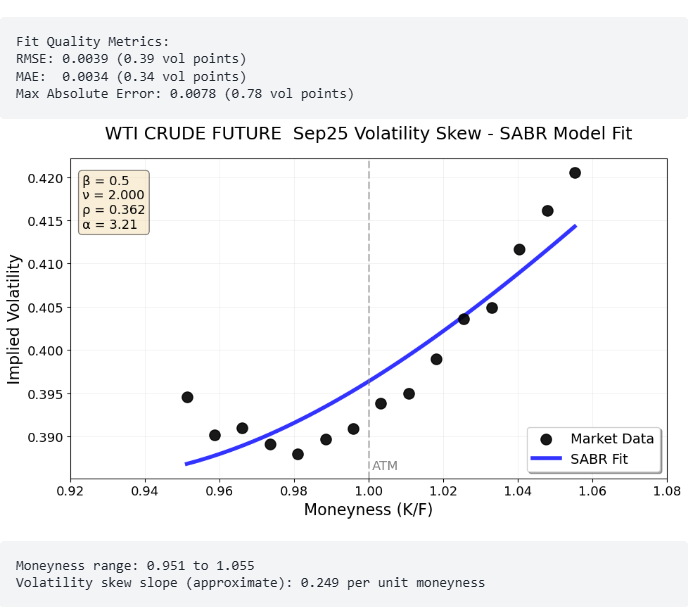
\includegraphics[width=0.85\linewidth,height=0.55\textheight,keepaspectratio]{figures/L7_3_c22_sabr_fit.png}\end{center}

The notebook fits SABR to a Bloomberg vol skew snapshot for WTI crude.
Calibrated $\beta = 0.5$. The fit recovers $\nu = 2.000$,
$\rho = 0.362$, $\alpha = \sigma_0 = 3.21$. RMSE on the fit is
$0.0039$ (about $0.4$ vol points), MAE about $0.34$ vol points.
Black dots are market quotes; blue line is the SABR curve. The fit is
visually clean and the few outliers (left wing) are characteristic
of low-liquidity strikes.
\end{keyblock}

The lecturer's framing on the live example was that the data set is
small --- ``I'm not going to get them across lots of strikes. That's
why we need something like SABR, because I am not going to see a lot
of market transactions across all these strikes.'' The Bloomberg
quote sheet has a handful of moneyness points (typically $\pm 100,
\pm 200, \pm 300$ bps), and SABR is the device that fills in the rest
of the curve consistently.

\begin{tipblock}
\textbf{Filling the gap.} A subtle methodological point the lecturer
raised: the data has to be \emph{synchronous}. ``I really can only fit
it on data that's synchronous, where I have quotes that are within
the same moment.'' Mixing a 10~am quote at strike $K_1$ with a 2~pm
quote at strike $K_2$ would attribute a market move to a strike
effect. In practice the desk pulls a single Bloomberg snapshot for the
entire chain. The same constraint applies to the implied-vol skew on
any market.
\end{tipblock}

\subsection{The vol path}\label{L7-sec:volpath}

\begin{keyblock}
\textbf{Cells~23--24 (\emph{Forward Price Scenarios} and
\emph{Volatility Surface Dynamics}).} \emph{(How the skew moves when
$F_0$ moves.)}

\begin{center}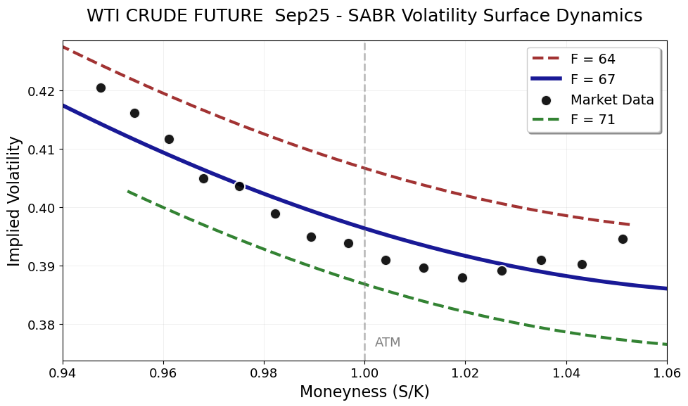
\includegraphics[width=0.85\linewidth,height=0.5\textheight,keepaspectratio]{figures/L7_3_c24_volpath.png}\end{center}

The plot fixes the calibrated $(\beta, \rho, \nu, \sigma_0)$ and
varies the forward price $F_0$. Each colored curve is the SABR
implied-vol curve at that forward level. The vertical dashed line at
$S/K = 1$ is the reference moneyness $S = K$. The market dots are
overlaid. \textbf{This is what SABR is for}: it predicts how the
implied-vol skew \emph{moves} as the underlying changes.
\end{keyblock}

The lecturer made the picture do the work. ``If the Fed funds rate
goes up to 440, red, I think all the implied vols are going to come
down.\ I think green is going to drop to red.\ \ldots\ This is exactly
what I need to make to have estimates of what I think that Vega
channel will be to my change in the option value.'' The colored
curves are SABR's prediction; for the homework they will be compared
to the empirical realized skew on subsequent days to assess fit.

\begin{tipblock}
\textbf{Filling the gap.} Two slices of this picture have very
different operational meaning, and the lecturer flagged this
explicitly:
\begin{itemize}
  \item \textbf{Vertical slice} (fix $K$, vary $F$): ``If I've bought
        a contract, I'm locked in on that strike, and I'm going to
        jump between curves on a vertical slice.'' This is the
        single-position augmented-delta calculation. The IV change
        I face on \emph{my} option is the gap between curves at
        $K = K_{\text{contract}}$.
  \item \textbf{ATM slice / vol path} (vary $F$, set $K = F$
        always): ``If I'm kind of looking at the market more
        generally as a market-maker, how do I think the implied vols
        are moving around?'' This traces the new ATM strike's IV as
        $F$ moves --- the ``where the action is'' curve. The notebook
        calls it the \emph{vol path}.
\end{itemize}
The two slopes need not even agree in sign. For a $1Y \to 4Y$
swaption the vertical and ATM slopes are usually similar; for index
options they can differ substantially.
\end{tipblock}

\begin{keyblock}
\textbf{Cell~25 (\emph{ATM Volatility Sensitivity to Forward Price
Changes}).} \emph{(Numerical sensitivity table.)}

\begin{center}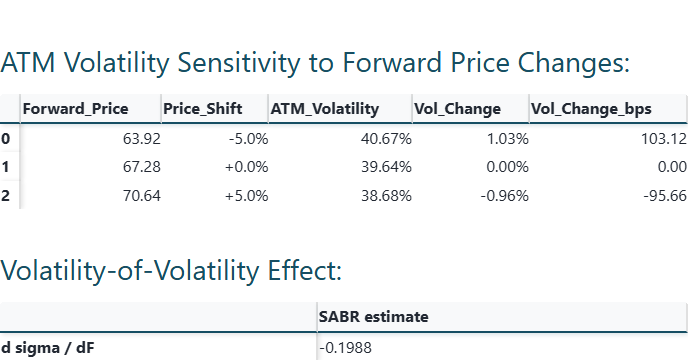
\includegraphics[width=0.7\linewidth,height=0.45\textheight,keepaspectratio]{figures/L7_3_c25_atm_sensitivity.png}\end{center}

For the WTI crude calibration, a $\pm 5\%$ shift in the forward price
moves the ATM implied vol by approximately $\pm 100$ bps:
\begin{itemize}
  \item $F_0 \times 0.95$: ATM vol $40.67\%$ ($+103$~bps vs.\
        baseline).
  \item $F_0 \times 1.00$ (baseline): ATM vol $39.64\%$.
  \item $F_0 \times 1.05$: ATM vol $38.68\%$ ($-96$~bps vs.\
        baseline).
\end{itemize}
The ``vol-of-vol'' effect, computed as the symmetric finite
difference $(\sigma^{\text{up}} - \sigma^{\text{down}})/(2\,\Delta F)$,
gives $d\sigma/dF \approx -0.1988$ per unit forward (in the
calibration's units) --- a clean negative slope at-the-money.
\end{keyblock}

\begin{checkpoint}
\textbf{My note.} A negative ATM-vol slope on WTI crude says: when
crude rallies, the at-the-money implied vol falls; when crude sells
off, it rises. This is the equity-style \emph{leverage effect} pattern
that gives $\rho < 0$ in equities, but here $\rho = +0.362$ in the
SABR fit. The two are not contradictory: $\rho$ is the
correlation between the forward and the \emph{instantaneous} vol
process, while the ATM-vol slope is a comparative-static across SABR
calibrations at different $F_0$ levels --- and at $\beta < 1$ the
$\sigma_0 / F_0^{1-\beta}$ rescaling drives much of the apparent ATM
slope, on top of the $\rho$ contribution. The lecturer's point in
the notebook is just to show that SABR \emph{has} a definite
prediction; whether the prediction is empirically right is what the
homework will assess.
\end{checkpoint}

\subsection{Tour across asset classes}\label{L7-sec:assettour}

The lecturer briefly walked through the SABR fits on several other
contracts (equity e-mini, treasury TY future, natural gas, NASDAQ).
The qualitative summary he wanted on the table:

\begin{itemize}
  \item \emph{S\&P~500 e-mini.} The vol-path picture has a mild
        positive slope: as the index rises, ATM implied vols
        \emph{rise} a little. This is at odds with the leverage-
        effect intuition for equities, and the lecturer was careful
        not to claim it as gospel: ``maybe SABR actually is a bad
        model for this asset.'' Beta-choice ($0.5$ vs $0$ vs $1$)
        materially changes the implied vol-path slope.
  \item \emph{10-year Treasury (TY) futures.} A slight negative
        slope at the money. Recall that an increase in the bond
        future's price corresponds to a decrease in rates, so the
        sign here, in rate-space, is positive --- ATM swaption-style
        vol rises as rates fall, which matches the broad fixed-income
        regularity that vol blows out on rate moves toward zero.
  \item \emph{Fed Funds, STIR, currency options.} SABR is heavily
        used. ``Almost entirely used in treasuries, STIR, and
        currency.''
\end{itemize}

\begin{checkpoint}
\textbf{My note.} The lecturer was cautious about SABR's equity
performance because the textbook-direction-flip he warned about does
empirically materialize: SABR with $\beta = 0.5$ and a positive $\rho$
will sometimes predict the implied-vol sheet to move \emph{up} when
equities rally, but observationally the equity vol surface usually
moves \emph{down} on rallies. Local-vol's directional implications
align with that data. SABR's strengths --- arbitrage-freeness and
correct fixed-income directional dynamics --- justify its place on
fixed-income desks; on equity desks the trade-offs go the other way.
\end{checkpoint}

\section{Internal consistency, arbitrage-freeness, and
homework}\label{L7-sec:closing}

A student question at the end of the lecture connected the strike-by-strike
mismatch between calls and puts in the market data to whether SABR's
fit could be tradable.

\begin{keyblock}
\textbf{The arbitrage-free property of SABR (and Black).}
SABR is internally consistent across put and call at the same strike:
the SABR-fitted implied vol is the \emph{same} number for both, by
construction. The implied vol is a property of the underlying SABR
process, not of the option type. Black has the same property. \\
A market quote that puts a put-vs-call gap on a single strike is
either liquidity-driven, friction-driven (American exercise, dividend
sensitivity in equities), or inventory-driven --- not a free lunch. A
big enough gap is, in principle, actionable; in practice, ``it's only
actionable if it's a big enough difference.''
\end{keyblock}

The lecturer's framing on this exchange was historical:
``If we could show up back in 1975 here, or if we could go to some
other option markets globally\ldots\ that is something I would say,
oh, we need to try to put in some trade ideas within three days.
Yeah, that's one of them. Let's look for big spreads in the put-call.
\ldots\ Maybe once in a while it is explained by market imbalance.
That's where we should be jumping in.'' The screening tool is the
quants' first contribution; the trade is what survives after
liquidity, frictions, and inventory have been priced in.

\subsection{Applications: collared floater and swaption augmented delta}\label{L7-sec:applications}

The lecturer previewed the homework at the end of class. Two
substantive new exercises layered on top of last week's work:

\begin{exerciseblock}
\textbf{Exercise (assigned, optional). Re-pricing the collared floater
with SABR-corrected skews.} The collared-floater case study used
\textbf{at-the-money} implied vols for the cap and floor legs, even
though by construction the cap is struck above the forward and the
floor below it. Calibrate SABR (using provided parameters or estimate
your own) to the relevant rate-option market. Re-extract the
skew-adjusted implied vol at $K_{\text{cap}}$ and $K_{\text{floor}}$,
then re-price the collared floater. Compare to the ATM-vol
baseline.
\end{exerciseblock}

\begin{exerciseblock}
\textbf{Exercise (assigned, primary). Augmented delta on the swaption
exercise.} The Lecture~6 swaption-pricing exercise priced the
$1Y \to 4Y$ swaption at strikes $\pm 100, \pm 200$~bps using the ATM
Black implied vol naively. Now use SABR to:
\begin{enumerate}[label=(\arabic*)]
  \item Calibrate SABR to the swaption skew at $1Y \to 4Y$.
  \item For each non-ATM strike, extract the skew-corrected implied
        vol and re-price the swaption.
  \item Compute the augmented delta
        \[
          \Delta_{\text{aug}} \;=\; \Delta_{\text{Black}}
             \;+\; \nu_{\text{Black}} \cdot \frac{\partial \sigma}{\partial F},
        \]
        where $\partial \sigma / \partial F$ is the SABR-implied
        vertical-slice derivative at that strike.
  \item Compare $\Delta_{\text{aug}}$ to $\Delta_{\text{Black}}$ and quantify the
        misstatement of the naive delta-hedge.
\end{enumerate}
\end{exerciseblock}

\begin{exerciseblock}
\textbf{Exercise (case-study followup, optional). Swaption vol
2020.} The lecturer flagged a related case using March~2020 swaption
data, where the skew moved sharply during the COVID rate cut. The
exercise traces SABR's predictions for the skew shift against the
actual realized shift, and asks whether the augmented delta would
have outperformed Black's delta as a hedge. The lecturer was still
deciding whether to assign this case or a smaller assortment of
exercises; the lecture handout will resolve which one ships.
\end{exerciseblock}

\subsection{Recap of what changed in our toolkit}\label{L7-sec:tk}

This lecture adds three new objects to the rate-derivatives toolkit:

\begin{enumerate}[label=(\arabic*)]
  \item \textbf{The volatility skew} as a first-class observable. Implied
        vol is not constant in $K$; the cross-section across strikes is
        a curve that absorbs everything Black ignores (liquidity,
        non-lognormal dynamics, risk aversion, market imbalance).
  \item \textbf{The Vega channel and the augmented delta.} The total
        derivative of an option's price with respect to the underlying
        is $\Delta_{\text{Black}} + \nu \cdot \partial\sigma/\partial F$,
        \emph{not} $\Delta_{\text{Black}}$. For a market-maker on a
        large book, ignoring the skew slope is the difference between
        a delta-neutral position and a hidden-duration bet.
  \item \textbf{The SABR model.} A two-factor stochastic-vol process
        for the forward and the vol with closed-form (asymptotic-
        expansion) implied-vol formula. Calibrated, not estimated,
        on $\beta$; remaining parameters $\sigma_0, \rho, \nu$ are
        identified from the ATM quote and the rest of the skew. The
        fitted SABR predicts the skew's response to underlying
        moves --- the data the desk needs for the augmented-delta
        hedge.
\end{enumerate}

The lens the lecturer wanted us to leave with: caps, floors, and
swaptions are the call/put toolkit on the swap and forward-swap
markets. Implied vol is the apples-to-apples quoting language, just
like YTM. The vol skew and the SABR fit on top of it are the next
layer of internal consistency that the desk needs to manage the
\emph{dynamics} of an options book, not just its static prices.
Lecture~8 will turn to the numerical-methods toolbox --- binomial
trees, finite-difference grids --- that the desk uses to price
American-style features (early exercise on callable bonds,
mortgage prepayments) where the closed-form Black machinery and
the SABR closed-form skew run out of analytic road.
